\chapter{Chapter 3 Supplementary Content}\label{app:ch3suppcontent}
\myappendices{Appendix \ref{app:ch3suppcontent}: Chapter 3 Supplementary Content}
\newpage

\section{Prediction Accuracy across all landmarks}\label{app:Chap}

\begin{table}[H]
\centering
\small
\caption{Per-landmark prediction accuracy of AutoAFIDs. Values represent the Euclidean Distance (ED) between predicted and ground truth landmark coordinates across 21 test subjects.}
\label{tab:autoafids_accuracy}
\begin{tabular}{lcccc}
\toprule
\textbf{Landmark} & \textbf{Median (mm)} & \textbf{IQR (mm)} & \textbf{Min (mm)} & \textbf{Max (mm)} \\
\midrule
AFID 1 & 0.42 & 0.29--0.69 & 0.04 & 1.53 \\
AFID 2 & 0.83 & 0.73--1.14 & 0.37 & 1.32 \\
AFID 3 & 0.90 & 0.65--1.09 & 0.36 & 2.06 \\
AFID 4 & 0.73 & 0.58--0.95 & 0.15 & 2.08 \\
AFID 5 & 0.80 & 0.60--1.12 & 0.29 & 2.46 \\
AFID 6 & 1.57 & 1.04--1.78 & 0.42 & 2.37 \\
AFID 7 & 1.26 & 0.86--1.55 & 0.24 & 2.39 \\
AFID 8 & 2.11 & 1.60--3.67 & 0.52 & 3.99 \\
AFID 9 & 1.41 & 1.07--2.43 & 0.51 & 3.99 \\
AFID 10 & 1.47 & 1.16--2.29 & 0.69 & 3.37 \\
AFID 11 & 0.72 & 0.48--0.84 & 0.25 & 1.23 \\
AFID 12 & 0.64 & 0.43--0.83 & 0.35 & 1.29 \\
AFID 13 & 0.93 & 0.68--1.11 & 0.38 & 1.60 \\
AFID 14 & 0.93 & 0.79--1.40 & 0.32 & 3.85 \\
AFID 15 & 2.00 & 0.97--3.30 & 0.26 & 5.28 \\
AFID 16 & 2.34 & 1.67--3.28 & 0.96 & 4.62 \\
AFID 17 & 2.38 & 1.19--2.61 & 0.32 & 3.99 \\
AFID 18 & 1.04 & 0.85--1.52 & 0.17 & 2.96 \\
AFID 19 & 1.27 & 1.02--1.56 & 0.14 & 2.83 \\
AFID 20 & 0.89 & 0.71--1.14 & 0.37 & 2.76 \\
AFID 21 & 1.32 & 0.70--1.73 & 0.47 & 4.03 \\
AFID 22 & 1.31 & 1.02--1.75 & 0.47 & 3.49 \\
AFID 23 & 1.16 & 0.53--1.69 & 0.10 & 3.31 \\
AFID 24 & 2.28 & 1.53--2.67 & 0.35 & 4.12 \\
AFID 25 & 2.28 & 1.66--3.04 & 0.64 & 3.59 \\
AFID 26 & 2.08 & 1.45--2.94 & 1.15 & 4.22 \\
AFID 27 & 1.47 & 0.80--2.10 & 0.21 & 3.46 \\
AFID 28 & 1.56 & 1.21--1.87 & 0.55 & 3.36 \\
AFID 29 & 1.79 & 1.38--2.46 & 0.70 & 3.61 \\
AFID 30 & 2.21 & 1.18--2.78 & 0.35 & 3.96 \\
AFID 31 & 1.19 & 0.91--1.63 & 0.34 & 2.98 \\
AFID 32 & 1.00 & 0.79--1.69 & 0.12 & 2.64 \\
\midrule
\textbf{All AFIDs} & \textbf{1.21} & \textbf{0.76--1.95} & \textbf{0.04} & \textbf{5.28} \\
\bottomrule
\end{tabular}
\end{table}

\newpage
\section{registration quality control file}
AutoAFIDs provides an optional registration quality control (QC) module that generates subject-level HTML reports to assess the fidelity of spatial normalization. For each subject, the tool computes standard summary statistics of landmark error, including minimum, maximum, mean, median, standard deviation, and interquartile range across all 32 anatomical fiducials. Visualizations include (i) slice-based qualitative review panels with crosshair overlays in sagittal, coronal, and axial views, (ii) a color-coded heatmap of per-landmark errors across x, y, z axes and Euclidean distance, and (iii) a 3D scatterplot showing the displacement between predicted subject landmarks and reference coordinates in stereotactic space. The report enables both quantitative inspection and visual verification of anatomical alignment and can be integrated into larger processing workflows for automated QC flagging.

The registration QC module in AutoAFIDs can be invoked as part of the BIDS-App command-line interface. To enable QC report generation, users must provide a directory containing their Lead-DBS derivative files. A typical invocation is shown below:

\begin{verbatim}
autoafids <BIDS_DIR> <DERIVATIVES_DIR> participant
--LEAD-DBS-DIR <PATH_TO_LEAD-DBS_Directory>
\end{verbatim}

This command runs the QC module on all subjects found in the BIDS directory, compares registered AFIDs to reference space, and saves the resulting HTML reports to the specified output directory. Each report includes per-subject error statistics, slice-wise visual inspection panels, a heatmap of landmark errors, and a 3D displacement plot. This functionality is integrated into the default workflow and designed for seamless use in automated pipelines.
\begin{figure}
    \centering
    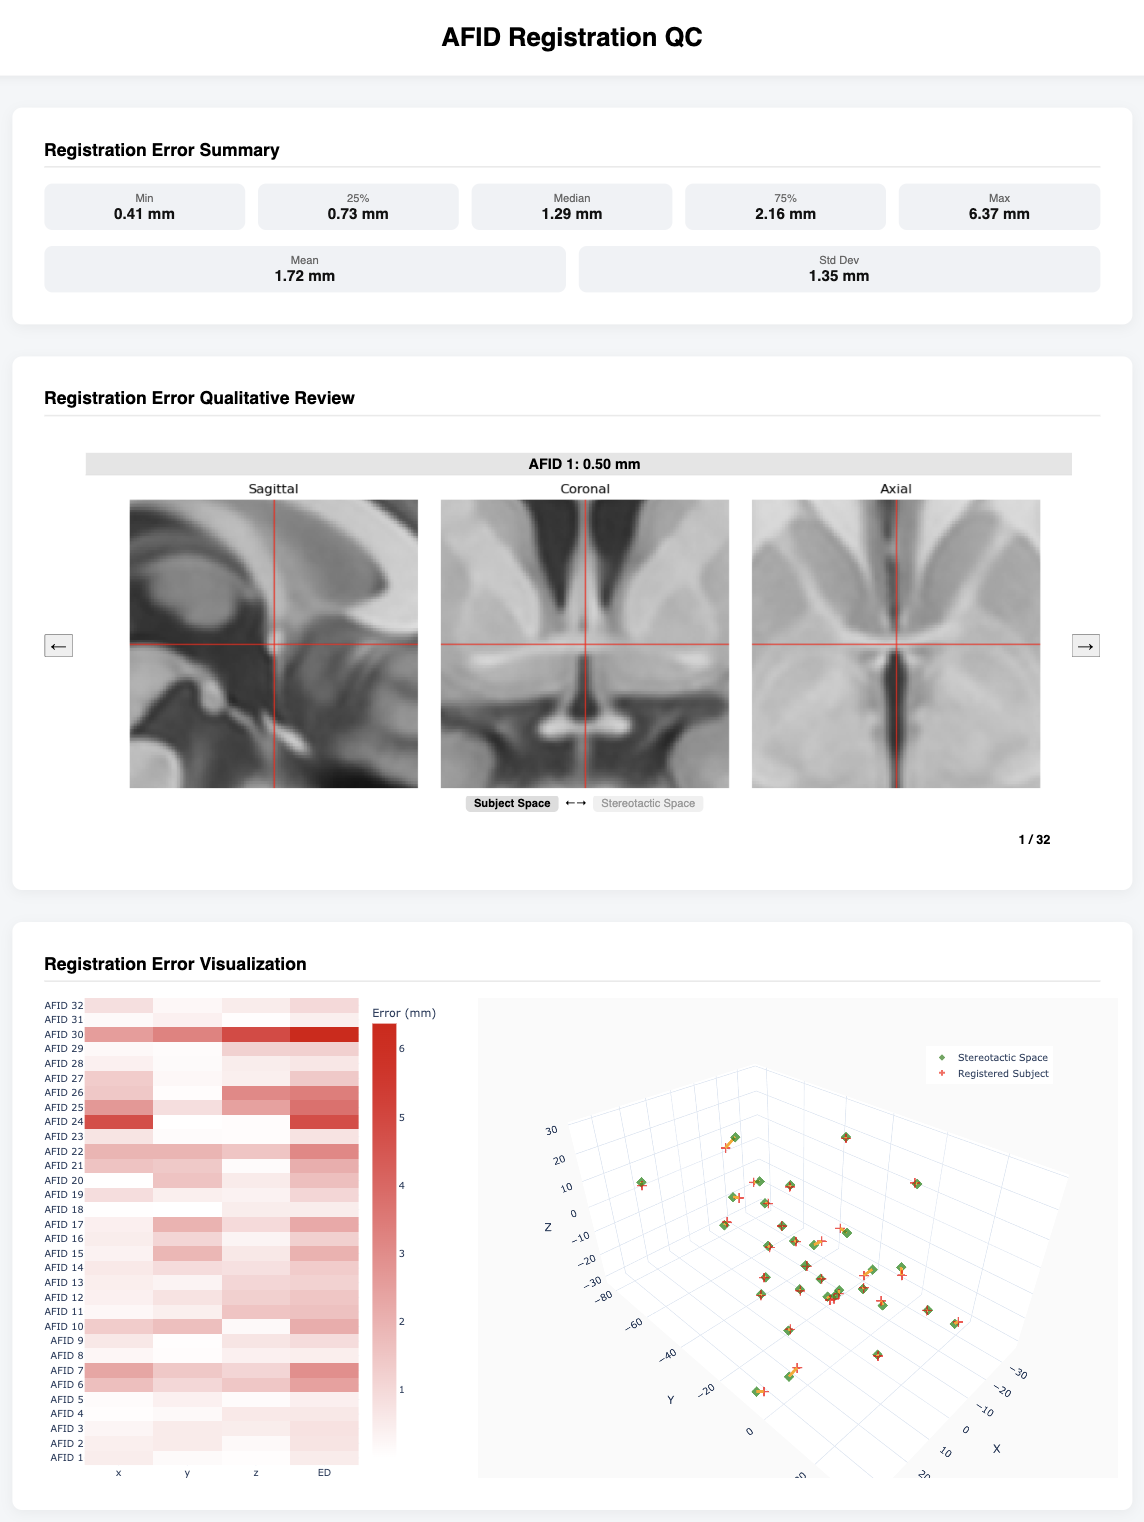
\includegraphics[width=0.95\linewidth]{figs/figuresupregqc.png}
    \caption{Example AutoAFIDs registration QC report for one subject.}
    \label{fig:figuresupregqc}
\end{figure}
\newpage
\section{AutoAFIDs Snakebids.yaml file}

\begin{minted}[fontsize=\small, bgcolor=bg, linenos, breaklines]{yaml}
bids_dir: "/path/to/bids/dir"
output_dir: "/path/to/output/dir"

force: True

debug: False
derivatives: False

analysis_levels: &analysis_levels
  - participant

targets_by_analysis_level:
  participant:
    - "all"

pybids_inputs:
  T1w:
    filters:
      suffix: T1w
      extension: .nii.gz
      datatype: anat
    wildcards:
      - subject
      - session
      - acquisition
      - reconstruction
      - run
    
  T2w:
    filters:
      suffix: T2w
      extension: .nii.gz
      datatype: anat
    wildcards:
      - subject
      - session
      - acquisition
      - reconstruction
      - run
  
  FLAIR:
    filters:
      suffix: FLAIR
      extension: .nii.gz
      datatype: anat
    wildcards:
      - subject
      - session
      - acquisition
      - reconstruction
      - run
  
  ct:
    filters:
      suffix: ct
      extension: .nii.gz
      datatype: anat
    wildcards:
      - subject
      - session
      - acquisition
      - reconstruction
      - run

parse_args:
#---  core BIDS-app options ---
  bids_dir:
    help: The directory with the input dataset formatted according to the BIDS standard.
  
  output_dir:
    help: The directory where the output files should be stored. If you are running
      group level analysis this folder should be prepopulated with the results of
      the participant level analysis.
      
  analysis_level:
    help: Level of the analysis that will be performed
    choices: *analysis_levels

  --participant_label:
      help: The label(s) of the participant(s) that should be analyzed. The label
            corresponds to sub-<participant_label> from the BIDS spec (so it does
            not include "sub-"). If this parameter is not provided, all subjects
            will be analyzed. Multiple participants can be specified with a space
            seperated list.
      nargs: "+"

  --exclude_participant_label:
      help: The label(s) of the participant(s) that should be excluded. The label
            corresponds to sub-<participant_label> from the BIDS spec (so it does
            not include "sub-"). If this parameter is not provided, all subjects
            will be analyzed. Multiple participants can be specified with a space
            sepearated list.
      nargs: "+"

  --acq:
      help: 'The acquisition sequence of the T1w image (e.g. MP2RAGE). (default: %(default)s)'
      default: MP2RAGE
      nargs: "?"

  --procprofile:
      help: 'Specify the profile and configration for preprocessing. (default: %(default)s)'
      choices: ['slow','medium','fast','superfast']
      default: 'fast'

  --norm:
      help: 'Specify the normalization scheme for images as a binary choice. {0 = z-score, 1 = min-max , 2 = tissue-based [notavailable]}. (default: %(default)s)'
      choices: ['0', '1']
      default: '0'  # Default to 0, which represents z-score normalization

  --res:
      help: 'Specify the resampling resolution (e.g. "100" for 1mm) for images, any resolution is supported but limited to isotropic resampling. (default: %(default)s)'
      default: '100'  # Default to 1 
    
  --modality: 
      help: 'Specify the modality to use (e.g., T1w, T2w, FLAIR, or CT).'
      default: 'T1w'
      choices:
        - T1w
        - T2w
        - FLAIR
        - ct

  --derivatives:
      help: 'Path(s) to a derivatives dataset, for folder(s) that contains multiple
        derivatives datasets (default: %(default)s) '
      default: false
      nargs: +

  --model:
      help: 'Type of machine learning model to apply.'
      default: 'default'
      required: false

  --enable-bids-validation:
    help: |
      Enable validation of BIDS dataset. BIDS validation would be performed
      using the bids-validator plugin (if installed/enabled) or with the pybids
      validator implementation (if bids-validator is not installed/enabled).
    dest: "plugins.validator.skip"
    action: "store_false"
    default: True

  --stereotaxy:
    help: 'Predict stereotactic target coordinates from output AFIDs. Also supplies AC-PC transform matrix (4x4) in the process.{STN = subthalamic nucelus, cZI = caudal zona incerta}'
    choices: ['STN','cZI']
    default: false
    required: false

  --fidqc:
    help: 'Generate *.html files for QC of AutoAFIDs outputs. (default: %(default)s)'
    dest: "fidqc"
    action: "store_true"  # Automatically sets to True when flag is used
    default: false        # Default to False when not used

  --LEAD-DBS-DIR:
    help: 'Path to a LEAD-DBS derivatives dataset, for folder(s) that contains multiple derivatives datasets (default: %(default)s) '
    default: false
    required: false
    type: str

  --FMRIPREP-DIR:
    help: 'Path to a fMRIPrep derivatives dataset, for folder(s) that contains multiple derivatives datasets (default: %(default)s) '
    default: false
    required: false
    type: str

  --workdir:
    help: |
      Folder for storing working files. If not specified, will be in "work/" subfolder 
      in the output folder. You can also use environment variables when setting the 
      workdir, e.g. --workdir '$SLURM_TMPDIR'.
    default: work
    type: str

#--- workflow specific configuration ---

# Nifti template
templatet1w: 'resources/tpl-MNI152NLin2009cAsym_res-01_T1w.nii.gz'
templatet1w_lead: 'resources/tpl-MNI152NLin2009bAsym_res-01_T1w.nii.gz'

# AFIDs fcsv template
fcsv: 'resources/dummy.fcsv'
fcsv_mni: 'resources/tpl-MNI152NLin2009cAsym_res-01_desc-groundtruth_afids.fcsv'
fcsv_mni_lead: 'resources/tpl-MNI152NLin2009bAsym_res-01_desc-groundtruth_afids.fcsv'

singularity:
  synthstrip: 'docker://freesurfer/synthstrip:1.3'
  synthsr: 'docker://mackenzieasnyder/synthsr:latest'

# It will be downloaded to ~/.cache/autoafids
resource_urls:
  default: 'files.osf.io/v1/resources/9fptg/providers/osfstorage/?zip='

#Stereotaxy models 
STN: 'resources/stereotaxy/STN.pkl'
cZI: 'resources/stereotaxy/cZI.pkl'
template_fcsv: 'resources/stereotaxy/target_template.fcsv'

plugins.validator.skip: False
root: results
workdir: null
\end{minted}
